\documentclass[]{article}
\usepackage[margin={1in}]{geometry}
\usepackage[spanish]{babel}
\usepackage{amsmath}
\usepackage{listings}
\usepackage{verbatim}
\usepackage{fancyhdr}
\usepackage[obeyspaces]{url}
\usepackage{graphicx}
\graphicspath{ {.} }


\pagestyle{fancy}
\fancyhf{}
\lhead{TC3041. Base de Datos Avanzadas \\ Actividad Diagnostico Complementaria}
\rhead{Andrés Alam Sánchez Torres (A00824854) \\ 15 de febrero de 2021}

\lstset{breaklines=true,
        language=SQL,
        extendedchars=true,
        basicstyle=\ttfamily\small,
        showstringspaces=false,
        literate={é}{{\'e}}1 {É}{{\'E}}1 
        } 


\begin{document}
    \setlength{\headheight}{23.10004pt}
    \addtolength{\topmargin}{-11.10004pt}

    \noindent
    \textbf{En base a la descripción siguiente soluciona las preguntas 1, 2, 3, 4 y ,5}
    
    \medspace
    
    \noindent
    Una compañía quiere mantener registro de los cursos de actualización que toman sus empleados. La
    información de los empleados incluye nombre, número de identificación y salario. Un empleado trabaja en
    solamente un departamento. Un departamento tiene un número de identificación único, un nombre y el número
    de identificación del administrador del dicho departamento. Un empleado puede tomar muchos cursos de
    actualización pero solo puede tomar un determinado curso una sola vez. Cada curso es identificado por un
    número de curso, un nombre descriptivo, y su duración en horas. Dado que un curso en particular puede ser
    ofrecido varias veces, la fecha que un empleado toma un curso también es registrado.
    Considera al instructor del curso como alguien ajeno a la compañía.

    \begin{enumerate}
        \item Dibuje el diagrama ER para esta empresa.
        
        \begin{center}
            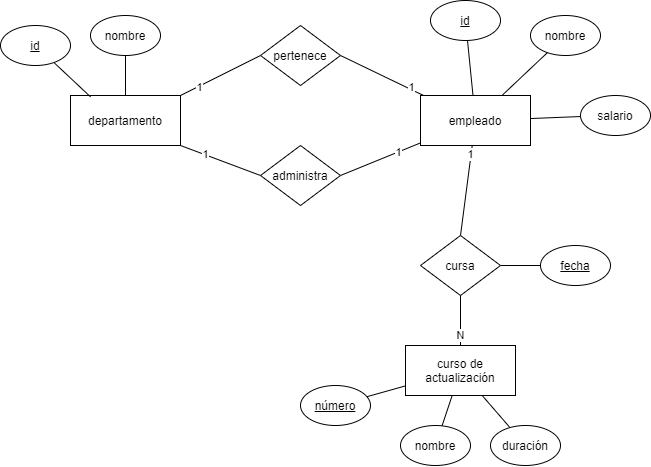
\includegraphics[scale=0.5]{er}
        \end{center}

        \item Traduzca su diagrama del inciso anterior en un Esquema Relacional (indique claramente las llaves
        primarias y foráneas)

        \begin{center}
            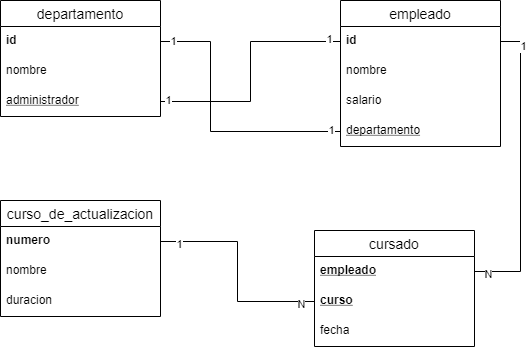
\includegraphics[scale=0.5]{relational}
        \end{center}

        \item Indique en que forma normal (y explique por qué) están sus relaciones
        
        Está en 3ra forma normal. Todas las columnas de todas las tablas contienen valores atómicos, las únicas dependencias
        que existen son con las llaves primarias y no hay dependencias transitivas.

        \item Basados en su esquema relacional del inciso anterior exprese la siguiente consulta en SQL.
        \begin{itemize}
            \item Liste el nombre de los empleados que han tomado el curso “Ética en el trabajo”
            \begin{lstlisting}
                select 
                    e.nombre 
                from 
                    empleado e,
                    cursado c,
                    curso_de_actualizacion curso
                where 
                    e.id = c.empleado and 
                    curso.nombre = "Ética en el trabajo"
            \end{lstlisting}
            \item Liste el nombre de los empleados que han tomado todos los cursos.
            \begin{lstlisting}    
                select 
                    e.nombre 
                from 
                    empleado e,
                    cursado c,
                where 
                    e.id = c.empleado
                group by
                    e.id
                having
                    count(*) = (
                        select count(*)
                        from curso_de_actualizacion
                        )
            
                \end{lstlisting}
        \end{itemize}
        \item Exprese las mismas consultas del inciso anterior pero ahora en Álgebra Relacional.
        
        \begin{itemize}
            \item Liste el nombre de los empleados que han tomado el curso “Ética en el trabajo”
            $$proyeccion \leftarrow empleado\ _{id}\bowtie_{empleado}\ cursado\ _{curso}\bowtie_{id}\ curso\_de\_actualizacion)$$
            $$\pi_{nombre}(\sigma_{nombre = "Etica\ en\ el\ trabajo"}(proyeccion)$$
            \item Liste el nombre de los empleados que han tomado todos los cursos.
            $$cursos \leftarrow numero\ \textbf{g}\ count\ numero\ (curso\_de\_actualizacion)$$
            $$\pi_{nombre}(\sigma_{empleado = cursos}(empleado\ \textbf{g}\ count\ empleado\ (cursado _{empleado}\bowtie_{id} empleado)))$$
        \end{itemize}
        
    \end{enumerate}
    

 

\end{document}